% Diagrama de secuencia — Ingesta de datos asistida por IA (estado 2026-09)
\documentclass[tikz, border=14pt]{standalone}
\usepackage[utf8]{inputenc}
\usepackage[T1]{fontenc}
\usepackage{helvet}
\renewcommand{\familydefault}{\sfdefault}
\usetikzlibrary{arrows.meta}

\tikzset{
  arr/.style={line width=0.8pt, -{Latex[length=2.3mm]}},
  ret/.style={line width=0.8pt, dashed, -{Latex[length=2.3mm]}},
  lbl/.style={font=\footnotesize\sffamily, fill=white, inner sep=1.2pt, align=center},
  head/.style={draw, line width=0.8pt, fill=black!12, minimum width=3.4cm, minimum height=0.9cm,
    align=center, font=\small\sffamily\bfseries},
}
\newcommand{\msg}[4]{\draw[arr] (#1,#3) -- (#2,#3) node[midway, above, lbl] {#4};}
\newcommand{\ret}[4]{\draw[ret] (#1,#3) -- (#2,#3) node[midway, above, lbl] {#4};}
\newcommand{\self}[3]{\draw[arr] (#1,#2) -- ++(0.5,0) -- ++(0,-0.4) -- ++(-0.5,0);
  \node[lbl, anchor=west, align=left] at (#1+0.6,#2-0.2) {#3};}
\newcommand{\frag}[6]{\draw[line width=0.7pt] (#1,#2) rectangle (#3,#4);
  \draw[line width=0.7pt, fill=white] (#1,#2) -- ++(1.0,0) -- ++(0,-0.3) -- ++(-0.15,-0.2) -- (#1,#2-0.5) -- cycle;
  \node[font=\footnotesize\sffamily\bfseries] at (#1+0.45,#2-0.25) {#5};
  \node[font=\footnotesize\sffamily, anchor=west] at (#1+1.1,#2-0.25) {#6};}
\newcommand{\els}[4]{\draw[line width=0.7pt, dashed] (#1,#2) -- (#3,#2);
  \node[font=\footnotesize\sffamily, anchor=west, fill=white, inner sep=1.5pt] at (#1+0.1,#2-0.25) {#4};}

\def\xU{0} \def\xA{4.2} \def\xB{8.8} \def\xS{13.4} \def\xC{18.0} \def\xD{22.6}

\begin{document}
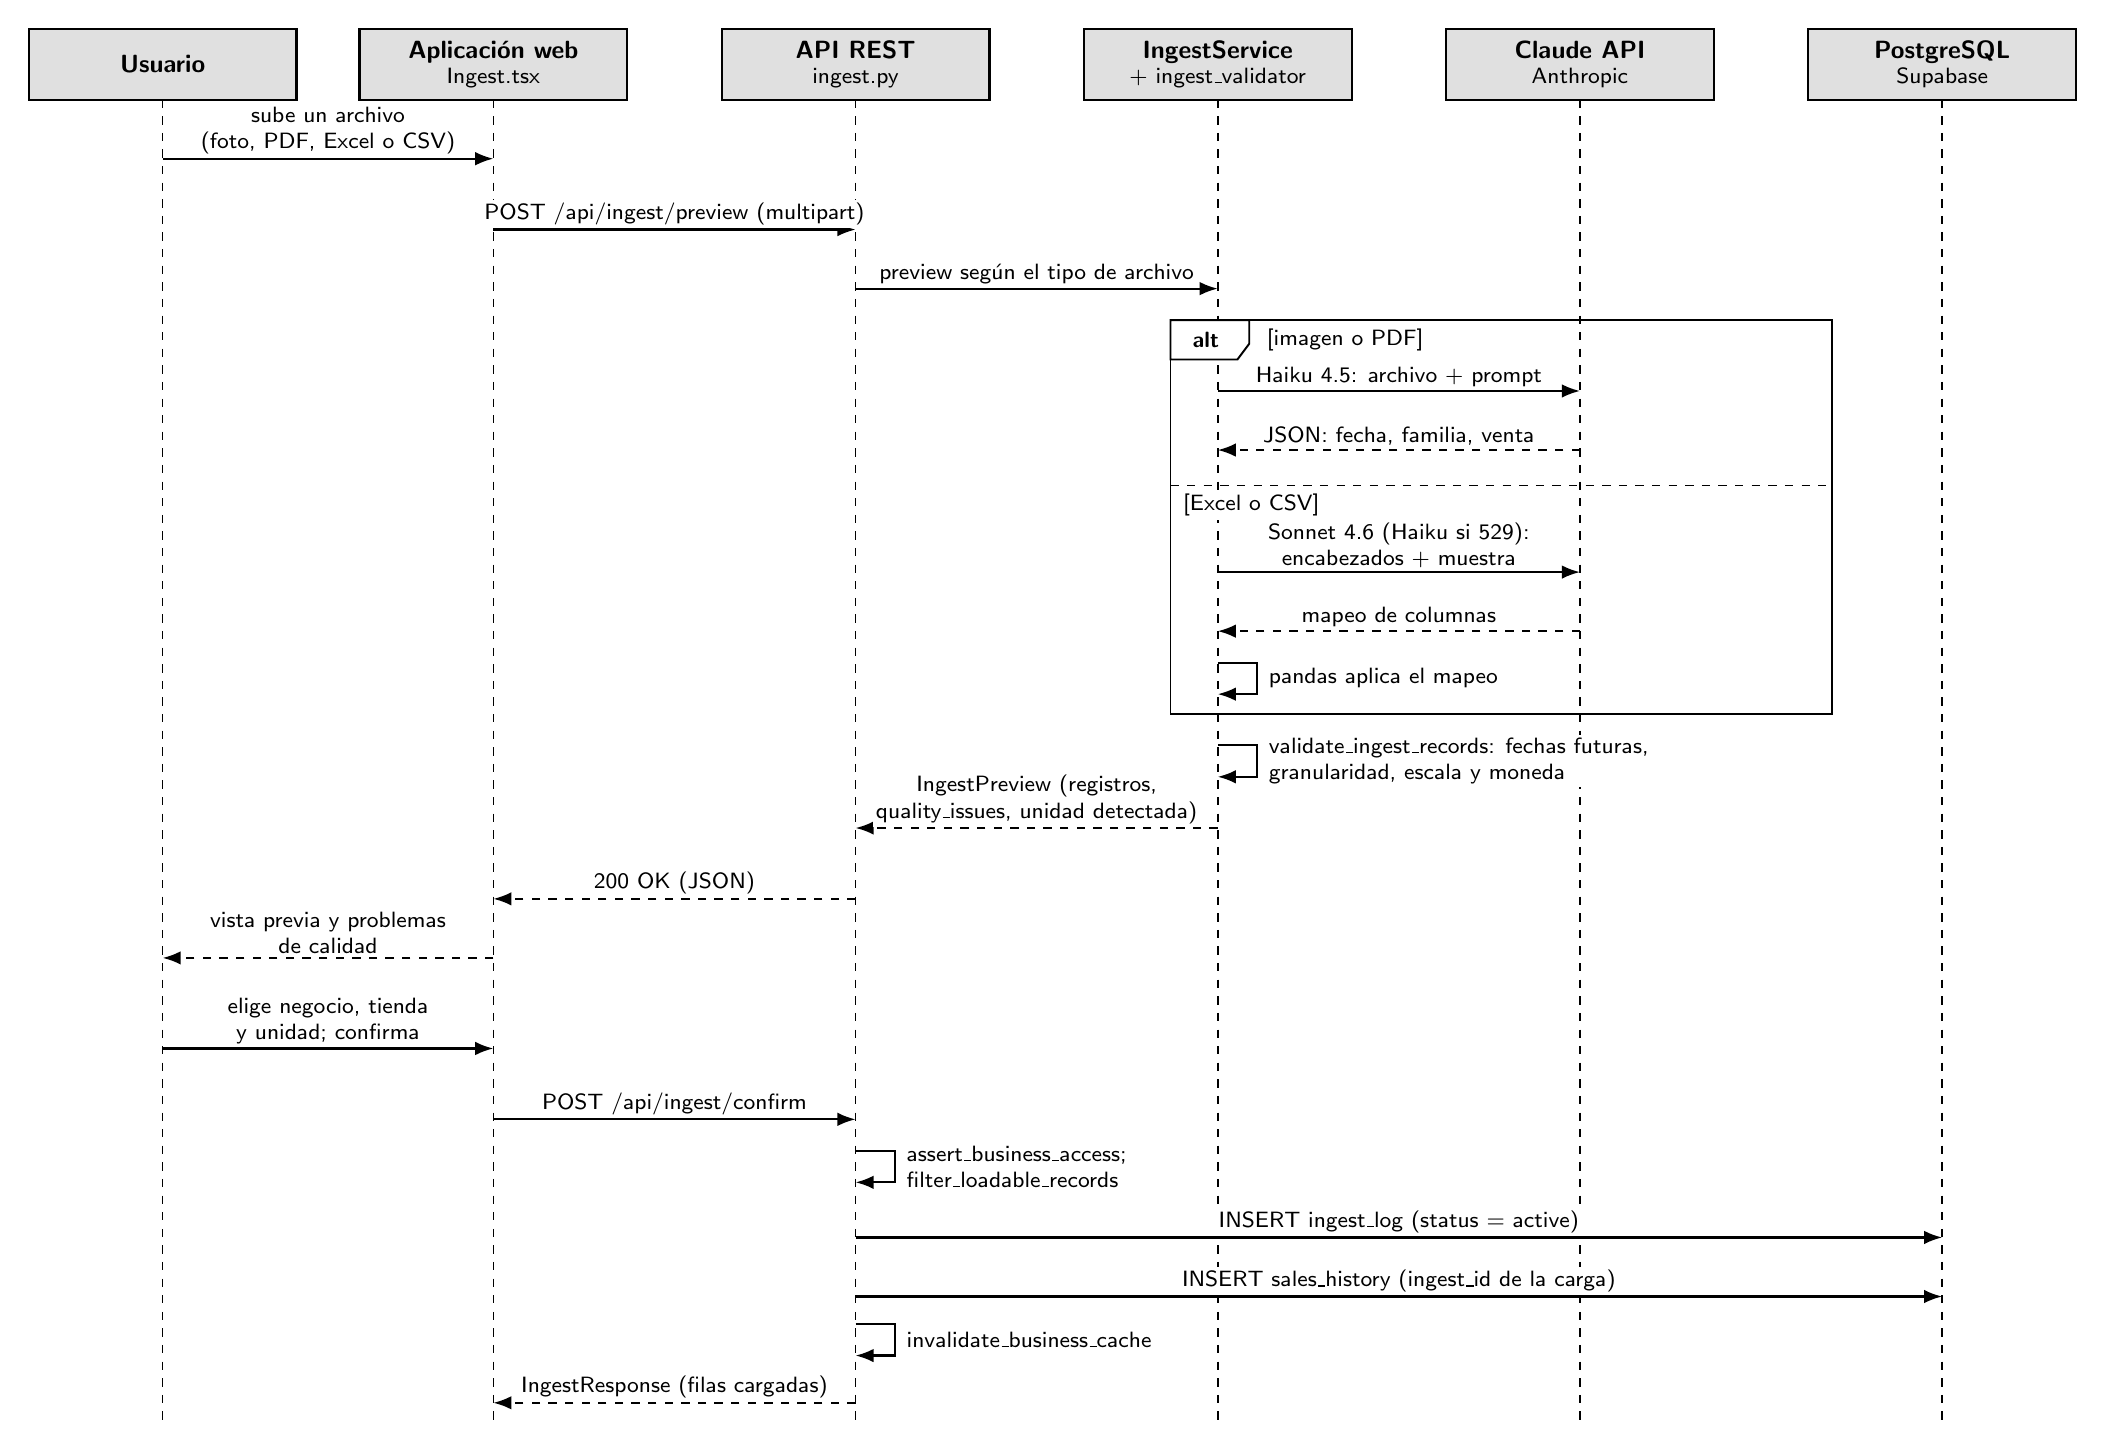
\begin{tikzpicture}[font=\sffamily]

\node[head] at (\xU,0) {Usuario};
\node[head] at (\xA,0) {Aplicación web\\[-2pt]{\footnotesize\mdseries Ingest.tsx}};
\node[head] at (\xB,0) {API REST\\[-2pt]{\footnotesize\mdseries ingest.py}};
\node[head] at (\xS,0) {IngestService\\[-2pt]{\footnotesize\mdseries + ingest\_validator}};
\node[head] at (\xC,0) {Claude API\\[-2pt]{\footnotesize\mdseries Anthropic}};
\node[head] at (\xD,0) {PostgreSQL\\[-2pt]{\footnotesize\mdseries Supabase}};
\foreach \x in {\xU,\xA,\xB,\xS,\xC,\xD} \draw[dashed, line width=0.6pt] (\x,-0.45) -- (\x,-17.3);

\msg{\xU}{\xA}{-1.2}{sube un archivo\\(foto, PDF, Excel o CSV)}
\msg{\xA}{\xB}{-2.1}{POST /api/ingest/preview (multipart)}
\msg{\xB}{\xS}{-2.85}{preview según el tipo de archivo}

\frag{12.8}{-3.25}{21.2}{-8.25}{alt}{[imagen o PDF]}
\msg{\xS}{\xC}{-4.15}{Haiku 4.5: archivo + prompt}
\ret{\xC}{\xS}{-4.9}{JSON: fecha, familia, venta}
\els{12.8}{-5.35}{21.2}{[Excel o CSV]}
\msg{\xS}{\xC}{-6.45}{Sonnet 4.6 (Haiku si 529):\\encabezados + muestra}
\ret{\xC}{\xS}{-7.2}{mapeo de columnas}
\self{\xS}{-7.6}{pandas aplica el mapeo}

\self{\xS}{-8.65}{validate\_ingest\_records: fechas futuras,\\granularidad, escala y moneda}
\ret{\xS}{\xB}{-9.7}{IngestPreview (registros,\\quality\_issues, unidad detectada)}
\ret{\xB}{\xA}{-10.6}{200 OK (JSON)}
\ret{\xA}{\xU}{-11.35}{vista previa y problemas\\de calidad}

\msg{\xU}{\xA}{-12.5}{elige negocio, tienda\\y unidad; confirma}
\msg{\xA}{\xB}{-13.4}{POST /api/ingest/confirm}
\self{\xB}{-13.8}{assert\_business\_access;\\filter\_loadable\_records}
\msg{\xB}{\xD}{-14.9}{INSERT ingest\_log (status = active)}
\msg{\xB}{\xD}{-15.65}{INSERT sales\_history (ingest\_id de la carga)}
\self{\xB}{-16.0}{invalidate\_business\_cache}
\ret{\xB}{\xA}{-17.0}{IngestResponse (filas cargadas)}

\end{tikzpicture}
\end{document}
